\documentclass[a4paper]{article}

\usepackage[utf8]{inputenc}
\usepackage[T1]{fontenc}
\usepackage{textcomp}
\usepackage[english]{babel}
\usepackage{amsmath, amssymb}
\usepackage{physics}


% figure support
\usepackage{import}
\usepackage{xifthen}
\pdfminorversion=7
\usepackage{pdfpages}
\usepackage{transparent}
\newcommand{\incfig}[1]{%
	\def\svgwidth{\columnwidth}
	\import{./figures/}{#1.pdf_tex}
}

\pdfsuppresswarningpagegroup=1
\title{ME 766 - High Performance Scientific Computing}
\begin{document}
\section*{Introduction}
Course content
\begin{itemize}
	\item Introduction to HPSC and scientific computing
	\item Processor performance, memory hierarchy, multi-core computing and vector computing
	\item Introduction  to parallel programming concepts and parallel algorithms
	\item Effective use of Bash scripting
	\item Effective use of tools like git, SVN, Mercurial etc
	\item OpenMP, MPI, GPGPU, Vector programming
	\item debuggers
	\item Performance analysis
	\item Numerical methods, applications of 
\end{itemize}

This course is all about making you a better researcher. It
is very hands on.
The processors keep changing every two years.
How to exploit hardware-level optimization techniques will also
change every two years. This course is targeted at those who are
pursuing a project - help them improve their code over there. So,
include this in your SoPs and course description. 

The biggest component of this course the project. All the best.
This project is a distillation of the professor's experience over
B.Tech. This man wants to \emph{teach}. So you better \emph{imbibe}. 

The traditional scientific method paradigms have been about observation 
$\to $ hypothesis $\to $ testing by experimentation and going back
to refine the hypothesis. Think Archimedes' eureka moment and
the fable of an apple falling on Newton's head.

A more concrete example would be the Higgs Boson discovery; the 
existence of the Higgs Boson was hypothesized much earlier.
The experiments at LHC set out to test this hypothesis and the
veracity of the standard model in general.

The computational modelling paradigm is much recent compared to the
traditional paradigms. It picked up during the second world war,
the Los Alamos project, for example

Alexei Krylov - general in the imperial soviet army (remember Krylov
subspaces and all that), his work led to important iterative methods
in linear algebra (typically systems with millions to billions of students).
Professor gave an example of computational fluid dynamics (CFD). I imagine
that a lot of examples will be from mechanical engineering.

Consider trying to solve for $\vec{x}$ in a linear system of size $n$

\begin{equation}
	\mathrm A \vec{x} = \mathrm B.
\end{equation}
If you do Gaussian elimination, you'll have an algo that goes as
$\mathcal{O}(n^3)$. Imagine if $n = 1\text{M}$. Unscalable.  Practical
applications using this method would be intractable even on the largest supercomputers.
Using iterative solvers would reduce the complexity to something 
like  $\mathcal{O}(n^2)$. If you're doing any serious computational
work, you will be using these methods instead of na\"ive Gaussian
elimination kind of methods.

\subsection*{Floating Point Operations (FLOPs)}
A FLOP is a binary operation between two floating point operands.
ENIAC was able to achieve 300 FLOPs per second (FLOPS, note the capitalisation). The ENIAC was used for writing artillery firing tables.
Some factors that would come in
\begin{itemize}
	\item Elevation of target
	\item Horizontal distance
	\item Aerodynamics of the shell
		\begin{itemize}
			\item wind direction
			\item geometry and weight of the shell
			\item density of air
			\item altitude
		\end{itemize}
	\item \ldots
\end{itemize}

ENIAC was insanely slow by modern computing standards. Head over to
\texttt{https://top500.org}. (AMD would have us believe that exascale
begins with their \texttt{Instinct MI100} GPUs). We are on the cusp of
the first exascale
machine. Thanks to Alexei Krylov's work.

The fastest supercomputer (SC) is Fugaku at RIKEN (Kobe, Japan). It
clocks a peak 537 Peta FLOPS, and consumes about 30 MegaWatts (as much
as a small town/city). IITB's SC, SpaceTime2, costs a few crores in
electricity alone. Fugaku is about 4 times more power efficient than
SpaceTime2. SpaceTime2 is also some four years old, and newer machines
are becoming more and more power efficient.

\subsection*{Application Areas}
\begin{itemize}
	\item CFD - sneeze and cough droplet simulations in these trying times
	\item Structural Mechanics - stresses, strains, deformations, fractures and all that
	\item Computational Electromagnetics - scattering of EM waves off e.g. an aircraft body (RADAR signature detection for military aircraft). Stealth
	\item Magnetohydrodynamics - e.g. molten ferromagnetic material flowing. Nuclear fusion reactors use a blanket of Lithium-Lead liquid
	\item Computational astrophysics - mostly exclusively computational, i.e. no experimental counterpart. You cannot really sit around to observe the evolution of a galaxy over a gajillion years
	\item Computational Finance - models made using partial differential equations (PDEs), usually involve all time scales (microtrading to long term investments et cetera)
	\item Molecular Dynamics (MD)
\end{itemize}

Computational science cannot completely replace experiments, of course.
You can explore the parameter space freely in computational models, and
then cherry pick promising results to be tested by experimental rigs.
``Computational science is the partial truth fully revealed. Experimental
science is the full truth partially revealed". When you make a computational
model, you have to start off with some simplifications.

\subsection*{What makes a good computational scientist}
\begin{itemize}
	\item Domain specific knowledge - obviously
	\item Programming proficiency - you should be able to write your models and math in code. You need to be able to use these large
		machines \emph{efficiently}.
	\item Excellent background in applied mathematics and numerical analysis
\end{itemize}

Your model on a machine should be able to procure a three-day prediction
in a few hours. It should also not run at some 30 megawatts just for
a three-day prediction for one city. We will use parallel computing
and serial computing optimization techniques.

Related to course logistics - the domain specific knowledge should
come from your end. This course is targeted at senior undergrads and 
postgrads. All the best.

Standard benchmarking programs do exist for supercomputers. E.g. LINPACK.

\section*{Why Parellel?}
So, by now we have learned that the high performance comes from
parallelization. Why can we not just go on making more and more
powerful sequential processing hardware?

\subsection*{Moore's Law}
VLSI circuits are a lot of transistors on a chip. We can only pack
so many transistors on a processor. What is the best that we can do?
One transistor per lattice site of the solid state material, if you
could get that level of control.

Point is that there is a physical limit to the number of transistors
that you can pack into a single chip. We are at the cusp of where
Moore's law will break down. Any year now.

\begin{figure}[h]
	\centering
	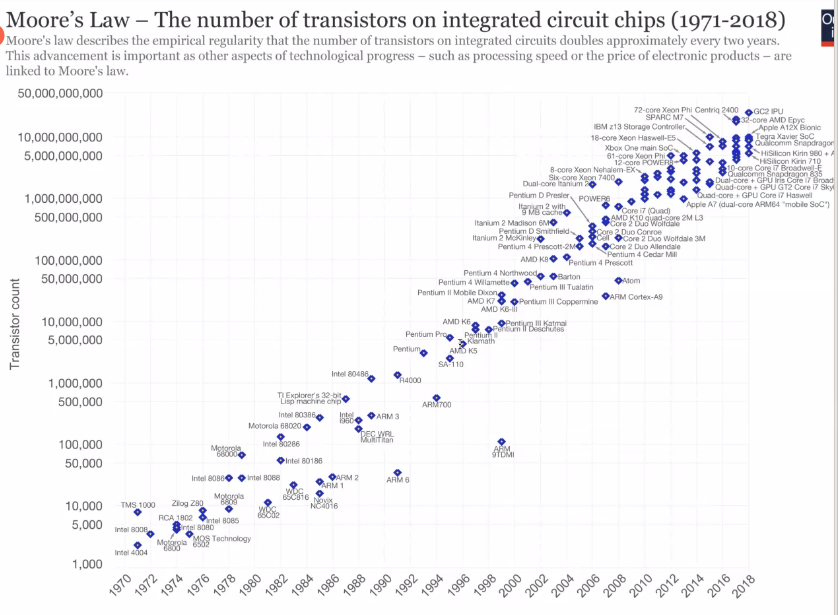
\includegraphics[width=0.8\textwidth]{figures/moore.png}
	\caption{Screenshot of a curve showing Moore's law}
	\label{fig:figures-moore-png}
\end{figure}

The MOSFET is a building block of these chips; each MOSFET functions
as a transistor.

\begin{figure}[h]
	\centering
	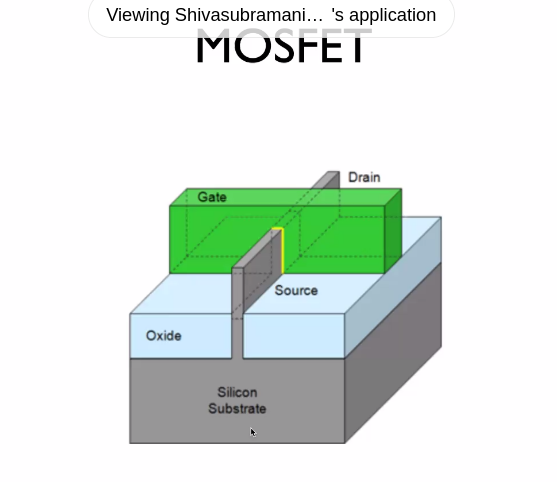
\includegraphics[width=0.8\textwidth]{figures/mosfet.png}
	\caption{MOSFET}
	\label{fig:figures-mosfet-png}
\end{figure}

Today in 2021, gate sizes in production are at 5 nanometers. The 
Apple M1 chips are built on a 5 nm tech. In research labs people 
already have 1 nm gates and sizes.

While Moore's law is holding up just fine (for now) Dennard scaling
has already broken down.

\begin{table}[h]
	\centering
	\caption{Dennard Scaling of MOSFETs (1974)}
	\label{tab:dennard}
	\begin{tabular}{c c}
	 Parameter & Factor\\
	 \hline
	 Dimension & l/k\\
	 Voltage & l/k\\
	 Current & l/k\\
	 Capacitance & l/k\\
	 Delay time & l/k \\
	 Power dissipation & l/k$^2$
	\end{tabular}
\end{table}

When you specify something like 1 volt, you know that it is not
exactly one volt; thermal motion of electrons et cetera will cause
fluctuations. At smaller scales, the transients and fluctuations
become comparable. 

Thermal losses also increase a lot as you go smaller and smaller.

\begin{figure}[h]
	\centering
	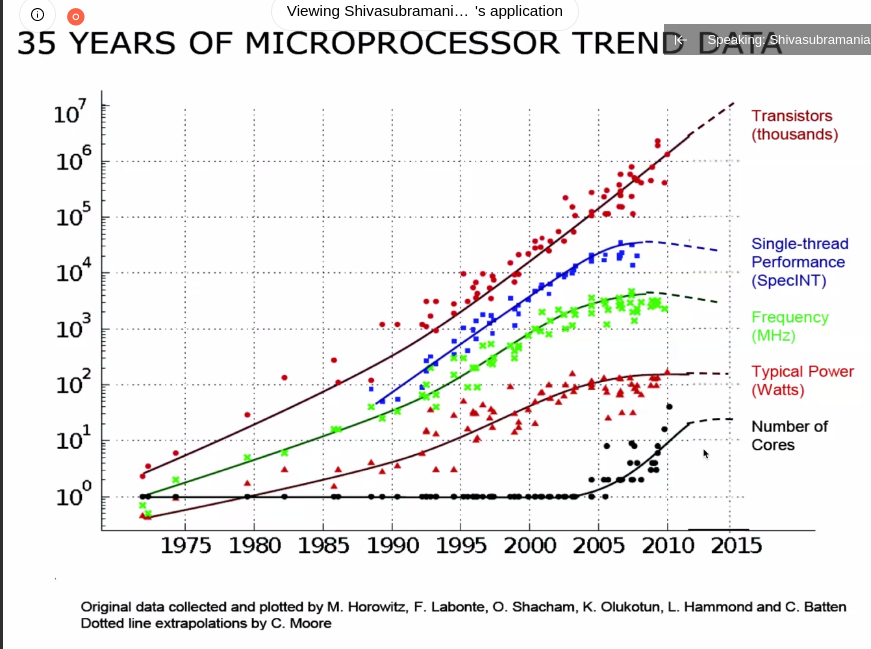
\includegraphics[width=0.8\textwidth]{figures/proctrends.png}
	\caption{35 Years of Microprocessor Trend Data}
	\label{fig:figures-proctrends-png}
\end{figure}

Essentially, single-thread performance, switching times and clock frequencies
et cetera are asymptoting, which means that single core performance
is becoming peak. You absolutely cannot run away from parallel
programming in the future.

Also, parallel programmers are needed because automatic parallelization
is very non-trtivial and is an area of active research.
An anecdote - around 2004-2005 some of the first dual core machines
were showing up, and people started thinking seriously about 
parallel programming. ``Why don't we invest in a compiler that does
automatic parallelization". They did, the code became slower by 50\%.

It is very easy to slow down the task by trying to parallelize it.

\subsection*{Amdahl's Law}
Your program will not be completely parallelizable; it will have both
serial and parallel components. If $P$ is the proportion of the program
that can be parallelized. Then the maximum speedup possible by parallelization
of the problem is 
\begin{equation} \label{amdahl}
	S(N) = \frac{1}{1 - P + \frac{P}{N}}
\end{equation}
where $N$ is the number of processors available at hand.

Consider a trivial problem like addition of an array of integers.
Sequentially, this is an $O(n)$. If we have 10 cores, then we
can partition the array into 10 parts, relegate each part to one
core. We end up with 10 partial sums, and then a single core
could sequentially add the partial sums to return the final sum.

So, we have $N = 10$. The original sum has $n$ floating point sum
operations. The parallel algorithm has $n/10 + 10$ floating point
summations (loosely speaking, I am assuming multiple FP adds occuring
in parallel as a single FP add). So, consider table \ref{tab:tabam}.
\begin{table}[h]
	\centering
	\caption{Amdahl's Law in action ($N = 10$) for an array sum}
	\label{tab:tabam}
	\begin{tabular}{c c c}
		$n$ &   $n/10 + 10$ & Speedup\\
		100 & 20 & 5 \\
		1000 & 110 & 9 \\
		10000 & 1010 & 9.9 \\
		\vdots & \vdots & \vdots
	\end{tabular}
\end{table}

This is a very rosy picture. You can lose the speedup because of 
communication overheads, latencies, load imbalance et cetera. 
Communication between different nodes in the system takes a significant
amount of time. Think about RAM v/s cache, RAM is much slower than
the speed at which your processor works. If you have to communicate
with the RAM frequently during a single process, R.I.P. Doesn't
matter how many cores you have, you have a major bottleneck.

Also, there is no golden test that tells you how much parallism your
sequential algo has. You have to take your sequential algo to the
whiteboard.

%%%%% TODO: complete the last example on Laplace equation
%%%%% Note that there is an intentional typo in this part of the slides
\end{document}
